\documentclass[12pt]{article}
\usepackage[total={7in, 10in}]{geometry}
\usepackage{amsmath,amsfonts,amsthm,amssymb, mathtools}
%\usepackage{xcolor}
\usepackage[dvipsnames]{xcolor}
\usepackage{graphicx,enumitem,parskip,textcomp}

\usepackage{twoopt}

\usepackage[spanish]{babel}


\spanishdecimal{.}
\setlength\parindent{0pt} 

\newcounter{ni}

\newcommand{\horrule}[1]{\rule{\linewidth}{#1}}
 
\usepackage{dirtytalk}

\usepackage{float}

\renewcommand{\familydefault}{\sfdefault} 
 


\title{	
\normalfont \normalsize 
\textsc{Universidad Nacional Autónoma de México} \\
\horrule{0.5pt} \\[0.4cm]
\Huge  

Reflexión final del proyecto de Ingeniería de Software 2022-2 \\
\horrule{2pt} \\[0.5cm] 
}


\author{ 
Demian Alejandro Monterrubio Acosta  \\
Nícolas Kano Chavira \\
Erik Federico del Río Pulido  \\
Emiliano Dominguez Cruz\\
Rodrigo García Padilla\\
} 
\date{\today} 

\begin{document}

\maketitle
 

\newpage


\section{Introducción}

\subsection{ Propósito del documento.}
En este documento se encuentran las especificaciones de la nueva página web del servicio musical FCmusic. Esta plataforma le dará al cliente acceso a toda su música desde la comodidad de su teléfono y/o computadora de manera rápida y sencilla. Este documento planea guiar el diseño e implementación de la plataforma.\\

\subsection{Resumen del Proyecto}
Nombre del proyecto:     FCmusic.

\textbf{Desarrolladores:}
\begin{itemize}
    
    \item del Río Pulido Erik Federico
    \item García Padilla Rodrigo
    \item Monterrubio Acosta Demian Alejandro 
    \item Kano Chavira Nícolas
    \item Domínguez Cruz Emiliano

\end{itemize}

\textbf{Usuarios finales:}
Miembros de la comunidad de la Facultad de Ciencias que quieran escuchar la música que tienen.\\

\subsection{Antecedentes}
Actualmente existen diversas aplicaciones especializadas en escuchar música, algunas de las más famosas son: Spotify, Apple music, Amazon music, Deezer, Google music, YouTube music, etc. La mayoría de estas aplicaciones son de pago, o requieren de una suscripción para usar todas las funcionalidades. 
A través de este proyecto vamos a replicar las características más importantes de estas aplicaciones e implementar un sistema gratuito que permite escuchar la música que se tiene compartida mediante archivos en google drive.\\


\subsection{ Propósito del sistema}

\textbf{1.1.1 Usuarios}\\
El sistema, (idealmente) estará disponible para cualquier usuario en la web (de la facultad de ciencias).

\begin{itemize}
    \item Usuarios: miembros de la comunidad de la Facultad de Ciencias, que quieran escuchar y compartir música previamente guardada en Google Drive.
    \item Administradores: administradores del sistema, encargados de dar mantenimiento.
\end{itemize}

\textbf{1.1.2 Ubicación}\\
El sistema, (idealmente) estará disponible para cualquier usuario en la web (de la facultad de ciencias).

\textbf{1.1.3 Necesidad}\\
Este sistema está hecho para poder acceder a las funcionalidades de cualquier sistema de música sin tener que pagar.

\section{Requerimientos del Cliente}

El cliente requiere un sistema para escuchar música; este sistema debe ser accesible desde cualquier navegador, pero también debe tener una aplicación móvil. El sistema deberá poder acceder a toda la música guardada en una carpeta de google drive, obtener su información, administrarla, reproducirla, y tener las funciones más importantes de las aplicaciones de reproducción de música (tipo Spotify, Amazon Music, etc.).
El sistema estará disponible para toda la comunidad de la facultad de ciencias.





\section{Objetivos}

\subsection{Objetivos Funcionales}

\subsubsection{Alta Prioridad}
El sistema podrá conectarse con Google Drive para extraer las canciones, guardar su información en la base de datos y utilizarlas. \\

El sistema deberá poder guardar (en una base de datos):
\begin{itemize}
    \item Canciones 
    \begin{itemize}
        \item Artista
        \item Nombre de canción
        \item Año de lanzamiento
        \item Género
        \item Duración
        \item Año de lanzamiento
        \item Álbum al que pertenece
        \item Estrellas
        \item Vistas
    \end{itemize}
    
    \item Usuarios:
    \begin{itemize}
        \item Nombre
        \item Correo electrónico
        \item Canciones que escuchan
        \item Canciones que les gustan
        \item Playlist
        \item Escuchado recientemente
    \end{itemize}
    
    \item Listas de reproducción
    \begin{itemize}
        \item Estado (público / privado)
        \item Índice de canción
    \end{itemize}
    
    \item Álbumes
    \begin{itemize}
        \item Nombre del álbum
        \item Canciones del álbum
    \end{itemize}

    \item Artistas
    \begin{itemize}
        \item Nombre del artista.
        \item Canciones del artista.
    \end{itemize}
    
    \item Estadísticas
\end{itemize} 

El sistema deberá tener listas de reproducción  y podrá ponerlas en aleatorio (shuffle). Las listas serán:
\begin{itemize}
    \item Personales
    \item Disponibles para todos
\end{itemize} 

El sistema contará con un sistema de búsqueda difusa para encontrar canciones. (Que autocomplete canciones o ayude en las mayúsculas y minúsculas para encontrar la canción). \\

El sistema podrá reproducir canciones, pausarlas, adelantarlas, retrocederlas, pasar a la siguiente canción o volver a la canción anterior. \\

El sistema tendrá un sistema de usuarios.


\subsubsection{Media Prioridad}

El sistema contará con un sistema de calificación con estrellas. \\

El Sistema tendrá un modelo de estadística a base de:
\begin{itemize}
    \item Calificación dada
    \item Canciones más escuchadas
    \begin{itemize}
        \item todo el tiempo
        \item en el momento (popularidad)
    \end{itemize}
\end{itemize}

El sistema tendrá una biblioteca local con canciones descargadas por el usuario.


\subsubsection{Baja Prioridad}
El sistema tendrá un sistema de recomendaciones.
\begin{itemize}
    \item Basado en año, género, artista.
\end{itemize}

El sistema tendrá un modelo de interacción entre usuarios, (i.e. Formar listas de reproducción compatibles de acuerdo a los géneros que ambos escuchan). \\

El sistema permitirá seguir a un artista o género
\begin{itemize}
    \item con un sistema de notificaciones. (i.e. Te avisa cuando hay una nueva canción de un artista o algún usuario crea una lista de reproducción)
\end{itemize}


\subsection{Objetivos No Funcionales}

\subsubsection{Fiabilidad}
\begin{itemize}
    \item El sistema intentará no colapsar, en caso de ocurrir un error se debe notificar al usuario sin cerrar la aplicación. 
\end{itemize}

\subsubsection{Usabilidad}
\begin{itemize}
    \item Un usuario que conoce cómo usar otro sistema de música será capaz de entender cómo usar este sistema en poco tiempo.
    
    \item Los administradores podrán usar eficientemente el sistema después de haber recibido un entrenamiento.
\end{itemize}


\subsubsection{Rendimiento}
\begin{itemize}
    \item El sistema será lo suficientemente bueno en rendimiento como para ser usado cómodamente por un usuario.
\end{itemize}


\subsubsection{Seguridad}
\begin{itemize}
    \item Las cuentas de los usuarios tendrán sus contraseñas protegidas para evitar el robo de su información.
    \item Tendremos la seguridad que ofrece Google.
\end{itemize}


\subsubsection{Compatibilidad}
\begin{itemize}
    \item El sistema funcionará en la mayoría de los navegadores más usados.
    \item El sistema podrá funcionar en la aplicación de dispositivos móviles. 
\end{itemize}


\subsubsection{Documentación de usuario en línea y ayuda}
\begin{itemize}
    \item El sistema tendrá un manual claro y documentado para el usuario, al cual se podrá acceder fácilmente desde la pantalla principal del sistema.
\end{itemize}


\subsubsection{Robusto}
\begin{itemize}
    \item El sistema será robusto respecto a errores.
\end{itemize}






\section{Arquitectura del Sistema}

Las tres partes más importantes del sistema son:
Frontend: la parte del sistema con la que el usuario interactúa.
Backend: la parte del sistema que se encarga de implementar todas las funcionalidades y  la comunicación entre las otras partes.
Base de datos: la parte que guarda toda la información y la consulta cuando sea necesario.

\begin{figure}[H]
\centering
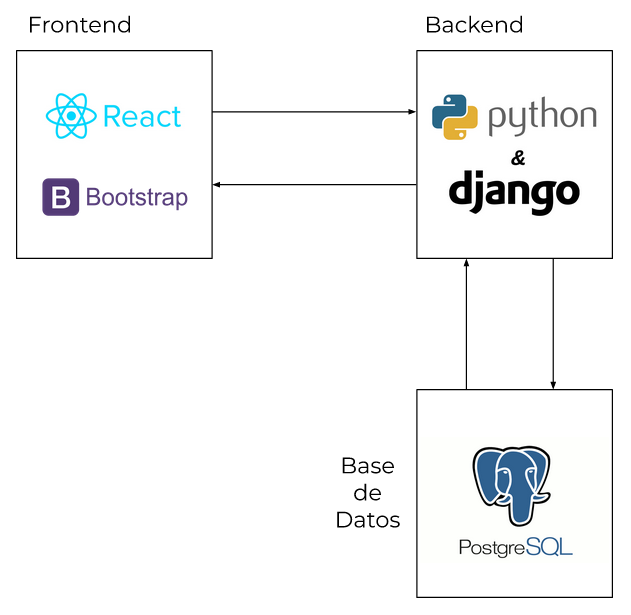
\includegraphics[scale=0.7]{Arquitectura.png}
\end{figure}

En este diagrama podemos ver la comunicación entre los módulos más importantes, y dentro de cada módulo, la tecnología que usaremos para su implementación. Para la base de datos usaremos PostgreSQL, para el backend usaremos Python con Django, y para el frontend usaremos React y Bootstrap. 
Estamos usando el modelo vista controlador.


\section{Modelos del Sistema}

\subsection{Modelo relacional de la base de datos:}

\begin{figure}[H]
\centering
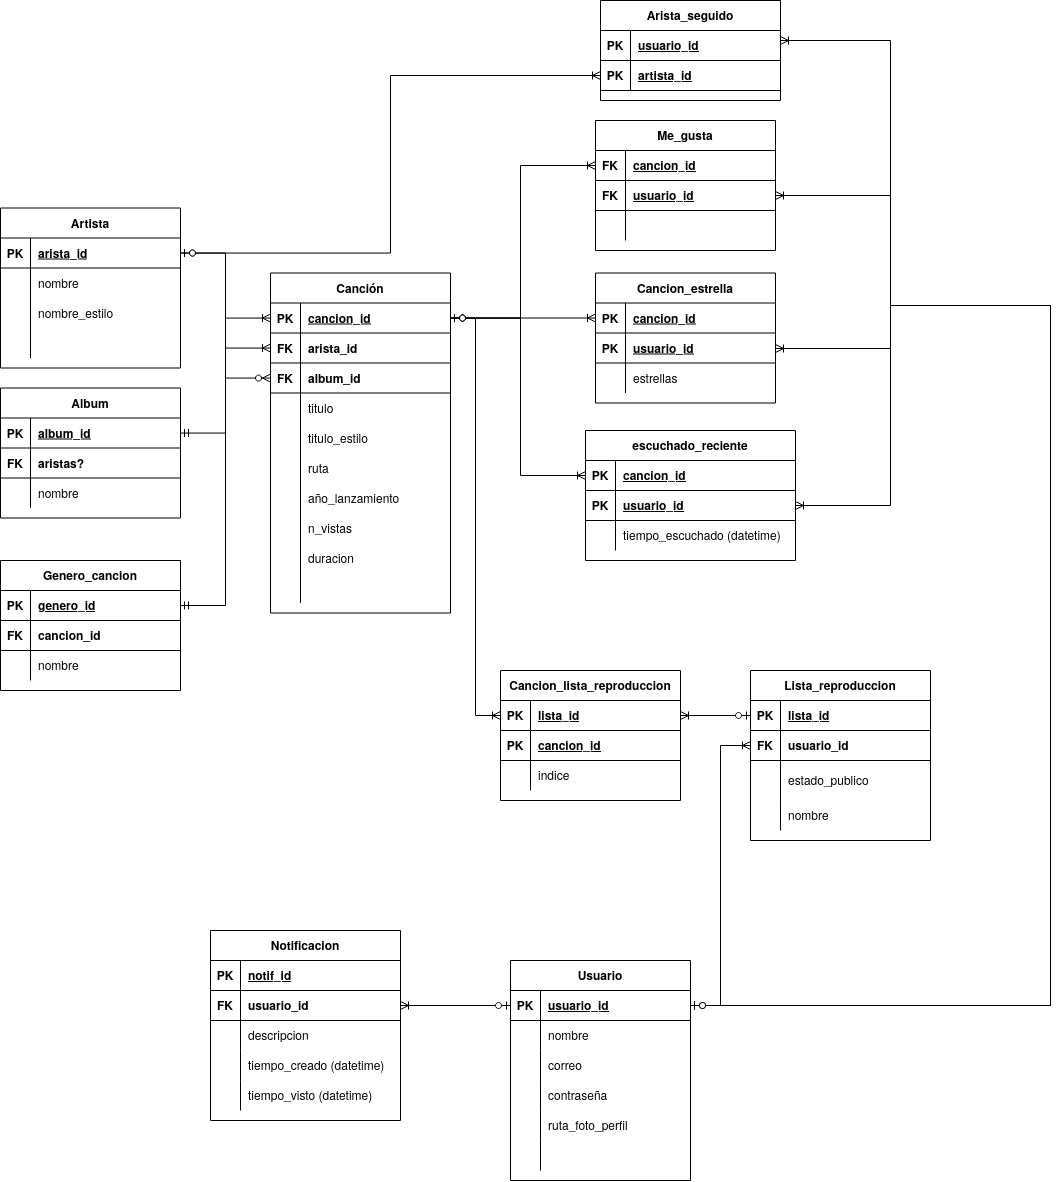
\includegraphics[width=16cm]{Modelo Relacional.png}
\end{figure}

Este modelo representa la información que guardaremos en la base de datos; cada cuadro es una tabla en la base de datos, que almacena la información listada. Las líneas que conectan las tablas indican la relación entre ellas. (Este modelo es tentativo).

\subsection{Modelo de clases del backend (simplificado):}

\begin{figure}[H]
\centering
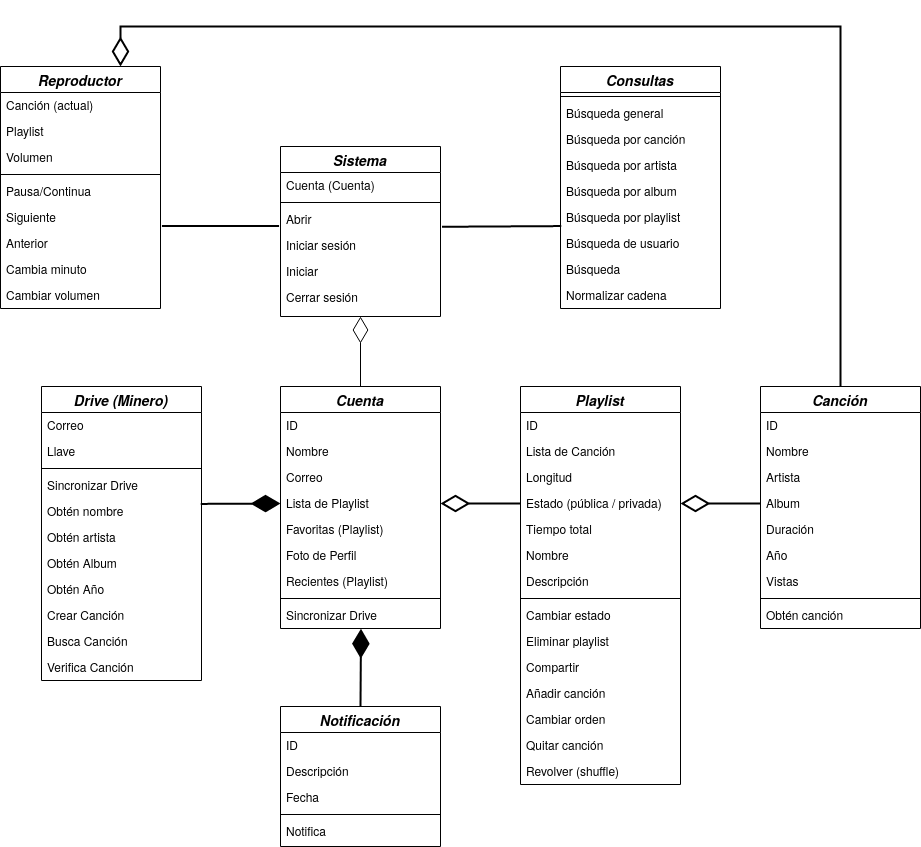
\includegraphics[width=16cm]{Diagrama de Clase Backend.png}
\end{figure}

Diagrama tipo UML (simplificado) de clases correspondiente al funcionamiento del backend. Las clases que harán que funcione el sistema están representadas por cuadros, sus atributos están en el primer rectángulo, y sus métodos en el segundo rectángulo.
Los nombres de los atributos y métodos no son los nombres finales del sistema, representan nombres descriptivos de lo que son / hacen.
El diagrama de clases corresponde a las funcionalidades de alta prioridad.


\section{Conclusiones}

El sistema que planeamos en este documento tiene las funcionalidades más importantes y esenciales para su funcionamiento; hay muchas otras características que podrían ser añadidas, aunque en principio no se planea que el sistema evolucione.
La principal deficiencia del sistema es que no cuenta con una base de datos con las canciones, depende de que estas canciones sean añadidas en Google Drive por los usuarios, esta decisión la tomó nuestro administrador (Canek), para que el sistema no tuviera problemas legales con el uso de música; si el sistema llegara a evolucionar, es bastante posible que esta característica se mantenga.
Como obtenemos la información de los archivos mp3, podríamos tener ciertas inconsistencias con la información real de las canciones; intentaremos que la información que mostremos de las canciones sea correcta; pero priorizaremos que el sistema sea funcional y consistente con sigo mismo.
Esperamos que el sistema cuente con todas las características planteadas y pueda estar disponible para la facultad de ciencias.


\section{Apéndice}

\subsection{Descripción de casos de uso (para casos selectos).}

\begin{table}[H]
\begin{tabular}{|l|p{0.77\linewidth}|lll}
\cline{1-2}
\multicolumn{1}{|c|}{Caso de Uso:} & \multicolumn{1}{c|}{Acceder a cuenta existente}                                                                                                                                                                                                                         &  &  &  \\ \cline{1-2}
Resumen:                           & Se inicia sesión en la cuenta del usuario existente.                                                                                                                                                                                                                    &  &  &  \\ \cline{1-2}
Flujo básico:                      & \begin{tabular}[c]{@{}l@{}}
1.Se redirige a la página de inicio de sesión de google.\\
2.Se ingresa su nombre de usuario o correo.\\ 
3.Se ingresa la contraseña correspondiente a la cuenta.\\ 
4.Se da click en el botón de acceder \\
5.El usuario entra a su cuenta
\end{tabular} &  &  &  \\ \cline{1-2}
Flujos alternativos:               & Si el usuario no recuerda su contraseña, google se encargará de restablecerla.                                                                                                                                                                                          &  &  &  \\ \cline{1-2}
Postcondiciones:                   & El usuario ingresa a su cuenta..                                                                                                                                                                                                                                        &  &  &  \\ \cline{1-2}
Reglas de negocio:                 & \begin{tabular}[c]{@{}l@{}}El usuario no debe crearse dos veces, \\es decir cada persona tiene derecho a una sola cuenta por correo.\\ Se debe cumplir con el dominio del correo.\end{tabular}                                                                            &  &  &  \\ \cline{1-2}
\end{tabular}
\end{table}








\begin{table}[H]
\begin{tabular}{|l|p{0.77\linewidth}|lll}
\cline{1-2}
Caso de Uso:         & Escuchar una lista de reproducción en “shuffle”.                                                                                                                                                                                                                                                                                                                                                                               &  &  &  \\ \cline{1-2}
Resumen:             & Se escucha una lista de reproducción en orden aleatorio.                                                                                                                                                                                                                                                                                                                                                                       &  &  &  \\ \cline{1-2}
Flujo básico:        & \begin{tabular}[c]{@{}l@{}}
1.El usuario se va a la sección “playlists”\\ 
2.El usuario entra en una lista de reproducción\\ 
3.El usuario selecciona el botón “shuffle”\\ 
4.La lista de reproducción se ordena de manera semi aleatoria.\\ 
5.El sistema empieza a reproducir la primera canción de la lista de reproducción\\ 
con el orden cambiado.\\ 
6.El sistema continúa reproduciendo canciones siguiendo el orden alterado.
\end{tabular} &  &  &  \\ \cline{1-2}
Flujos alternativos: & \begin{tabular}[c]{@{}l@{}}
4.5. El usuario puede volver a seleccionar el botón shuffle          las veces que quiera.\\
7.Si ya se escucharon todas las canciones de la lista, el sistema deja de reproducir\\ canciones.\end{tabular}                                                                                                                                                                                             &  &  &  \\ \cline{1-2}
Precondiciones:      & \begin{tabular}[c]{@{}l@{}}El usuario está dentro del sistema.\\ El usuario está en la página principal del sistema.\\ El usuario tiene al menos una  lista de reproducción.\end{tabular}                                                                                                                                                                                                                                      &  &  &  \\ \cline{1-2}
Postcondiciones:     & El usuario escucha su lista de reproducción en un orden semialeatorio.                                                                                                                                                                                                                                                                                                                                                         &  &  &  \\ \cline{1-2}
Reglas de negocio:   & Seleccionar el botón shuffle no afectará a ninguna lista de reproducción que tenga guardado el usuario, no creará ni eliminará nada; y si el usuario vuelve a la página principal, la lista volverá a estar ordenada como antes del “shuffle”.                                                                                                                                                                                 &  &  &  \\ \cline{1-2}
\end{tabular}
\end{table}






\begin{table}[H]
\begin{tabular}{|l|p{0.77\linewidth}|lll}
\cline{1-2}
Caso de Uso:         & Agregar una canción a una playlist.                                                                                                                                                                                                                                                                                                                              &  &  &  \\ \cline{1-2}
Resumen:             & Se modifica una playlist existente para agregar una canción.                                                                                                                                                                                                                                                                                                     &  &  &  \\ \cline{1-2}
Flujo básico:        & \begin{tabular}[c]{@{}l@{}}1. El usuario elige una canción, ya sea que la esté escuchando o la haya buscado.\\ 2. El usuario hace click en el botón “agregar a playlist”.\\ 3. El sistema muestra una lista de playlist candidatas para agregar.\\ 4. El usuario selecciona la playlist a cuál agregar.\\ 5. El sistema agrega la canción al final de la playlist.\end{tabular} &  &  &  \\ \cline{1-2}
Flujos alternativos: & \begin{tabular}[c]{@{}l@{}}5. Si la canción ya se encuentra en el playlist no se\\           agrega una copia.\end{tabular}                                                                                                                                                                                                                                      &  &  &  \\ \cline{1-2}
Precondiciones:      & \begin{tabular}[c]{@{}l@{}}El usuario ha ingresado a su cuenta.\\
Debe de existir una playlist en la cuenta del usuario\end{tabular}                                                                                                                                                                                                                            &  &  &  \\ \cline{1-2}
Postcondiciones:     & La canción ahora se encuentra en el playlist seleccionado                                                                                                                                                                                                                                                                                                        &  &  &  \\ \cline{1-2}
Reglas de negocio:   &                                                                                                                                                                                                                                                                                                                                                                  &  &  &  \\ \cline{1-2}
\end{tabular}
\end{table}







\begin{table}[H]
\begin{tabular}{|l|p{0.77\linewidth}|lll}
\cline{1-2}
Caso de Uso:         & Un usuario sube una nueva canción al sistema                                                                                                                                                                                                                                                                                                                                                                                                                                                                                                                                                                                                                            &  &  &  \\ \cline{1-2}
Resumen:             & Este caso de uso le permite a un usuario añadir una nueva canción al sistema para que se pueda escuchar.                                                                                                                                                                                                                                                                                                                                                                                                                                                                                                                                                                &  &  &  \\ \cline{1-2}
Flujo básico:        & \begin{tabular}[c]{@{}l@{}}
1. El usuario quiere subir una canción al sistema.\\
2. El usuario sube la canción a su carpeta de google drive.\\
3. El usuario inicia sesión en el sistema.\\
4. El usuario se va a la sección de su cuenta.\\
5. El usuario presiona el botón de sincronizar.\\
6. El sistema automáticamente encuentra la canción nueva en su cuenta de\\
   drive y  saca la información de la canción usando los meta-datos del mp3.\\ 
7. El sistema presenta una pantalla de “sincronización exitosa”.\\
8. La canción ya está dentro del sistema y se puede buscar en el buscador.\\
9. El sistema manda una notificación al usuario con las nuevas canciones\\ añadidas.

\end{tabular} &  &  &  \\ \cline{1-2}
Flujos alternativos: & \begin{tabular}[c]{@{}l@{}}
6. El usuario corrige cualquier dato incorrecto.\\       7.   El usuario da aceptar para guardar los cambios.\\ 10. La canción se sube exitosamente.
\end{tabular}                                                                                                                                                                                                                                                                                                                                                                                                                                                                               &  &  &  \\ \cline{1-2}
Precondiciones:      & El usuario puede iniciar sesión en el sistema.                                                                                                                                                                                                                                                                                                                                                                                                                                                                                                                                                                                                                          &  &  &  \\ \cline{1-2}
Postcondiciones:     & Como la canción ya está en el sistema, ya se puede usar para cualquier otro caso en el que se necesite.                                                                                                                                                                                                                                                                                                                                                                                                                                                                                                                                                                 &  &  &  \\ \cline{1-2}
Reglas de negocio:   & Las canciones ya existentes, ya no se guardan. Es la misma canción si es del mismo artista y tiene el mismo nombre.                                                                                                                                                                                                                                                                                                                                                                                                                                                                                                                                                     &  &  &  \\ \cline{1-2}
\end{tabular}
\end{table}

\section{Resultados y Reflexiones:}

La versión final del proyecto no cumplió con los requerimientos descritos en este documento; a continuación presentaremos una reflexión grupal e individual sobre el proyecto y por qué no pudimos cumplir con las expectativas.

\subsection{Generales}
A partir de una discusión del equipo llegamos a que, de manera general, estas son las razones por las que no acabamos el proyecto:

\begin{itemize}
    \item Integración tardía de componentes:
        Se dejó la unión de los componentes al final, cosa que impidió que el producto final se lograra, subestimando la complejidad del despliegue web del mismo, así como una base de datos en la nube.
    \item Fragmentación de los integrantes:
        Los primeros elementos del equipo terminaron dejando la materia, cosa que evitó la continuidad del proyecto, y a su vez trajo conflictos internos de decisión de temática del mismo.
    \item Falta de comunicación entre el equipo:
        Poca comunicación entre integrantes, lo cual trajo incertidumbre entre los avances significativos de cada uno y conciencia de otros integrantes de los mismos.
    \item Mala técnica de organización:
        Carencia de técnicas vistas durante el curso tales como SCRUM, debido a que aunque se implementaron en un inicio, terminaron por abandonarse debido a que no resultaron orgánicas, las cuales hubieran permitido llevar un ritmo constante de trabajo.
        
    \item Falta de experiencia:
        Nuestro equipo carecía de personas que hubieran llevado la realización de un proyecto de principio a fin (en proyectos web), por lo cual no sabiamos como abordar el proyecto, ni sus componentes y hubo detalles no previstos hasta una etapa tardía del desarrollo.
    \item Implementación tardía del proyecto:
        Se dejó la parte de las tecnologías del proyecto para el final, lo cual trajo problemas con la estimación de tiempos y por tanto finalización.
    \item Falta de buenas de prácticas de ingeniería de software:
        Carencia de uso de interfaces para división del trabajo, y de herramientas coolaborativas.
\end{itemize}

\vspace{1cm}
Individualmente, estas son las reflexiones que tenemos:

\subsection{Demian}
\subsection{Nícolas}
\subsection{Erik}
\subsection{Emiliano}
\subsection{Rodrigo}

\end{document}